\vspace{1.5pc}
\section[Domain dan Data Penelitian]{Domain dan Data Penelitian}
\begin{spacing}{1.5}
	\subsection[Domain Penelitian]{Domain Penelitian}
	Penelitian ini mengkaji hubungan antara IOD, variabel oseanografi (arus, temperatur, salinitas, MLD, Chl-a, fluks air tawar, fluks panas bersih) dan meteorologi (laju presipitasi dan angin) di Samudera Hindia dengan koordinat ($0^\circ-24.6^\circ$ N) dan ($78.2^\circ-105^\circ$ E) (lihat Gambar \ref{fig:domain}).

	\subsection[Data Penelitian]{Data Penelitian}
%	\vspace{-1pc}
	Data yang digunakan dapat dilihat secara lengkap dalam Tabel \ref*{tab:data}.
	\begin{table}[H]
		\centering
		\caption{Rangkuman data penelitian}
		\label{tab:data}
		\begin{tabular}{|l|l|l|l|l|}
			\hline
			No & Data               & Periode   & Sumber      & Referensi \\ \hline
			1  & IOD                & 1994-2021 & AUSS        & AUSS      \\ \hline
			2  & Arus               & 1994-2021 & CMEMS/HYCOM & AUSS      \\ \hline
			3  & Temperatur laut    & 1994-2021 & CMEMS/HYCOM & AUSS      \\ \hline
			4  & Salinitas          & 1994-2021 & CMEMS/HYCOM & AUSS      \\ \hline
			5  & MLD                & 1994-2021 & CMEMS       & AUSS      \\ \hline
			6  & Chl-a              & 1994-2021 & CMEMS/MODIS & AUSS      \\ \hline
			7  & Fluks air tawar    & 1994-2017 & J-OFURO3    & AUSS      \\ \hline
			8  & Fluks panas bersih & 1994-2017 & J-OFURO3    & AUSS      \\ \hline
			9  & Laju presipitasi   & 1994-2021 & NCEP/NCAR   & AUSS      \\ \hline
			10 & Angin              & 1994-2021 & NCEP/NCAR   & AUSS      \\ \hline
		\end{tabular}
	\end{table}
	\subsection[Pengumpulan Data]{Pengumpulan Data}
	Data dalam Tabel \ref{tab:data} merupakan data yang tersedia secara gratis dan bersifat terbuka. Data ini dapat diunduh secara langsung pada website penyedia data ataupun menggunakan koding. Koding dengan bahasa \textit{Shell script} (terminal Linux) disajikan dalam Lampiran 1.
	
	\begin{figure}[H]
		\centering
		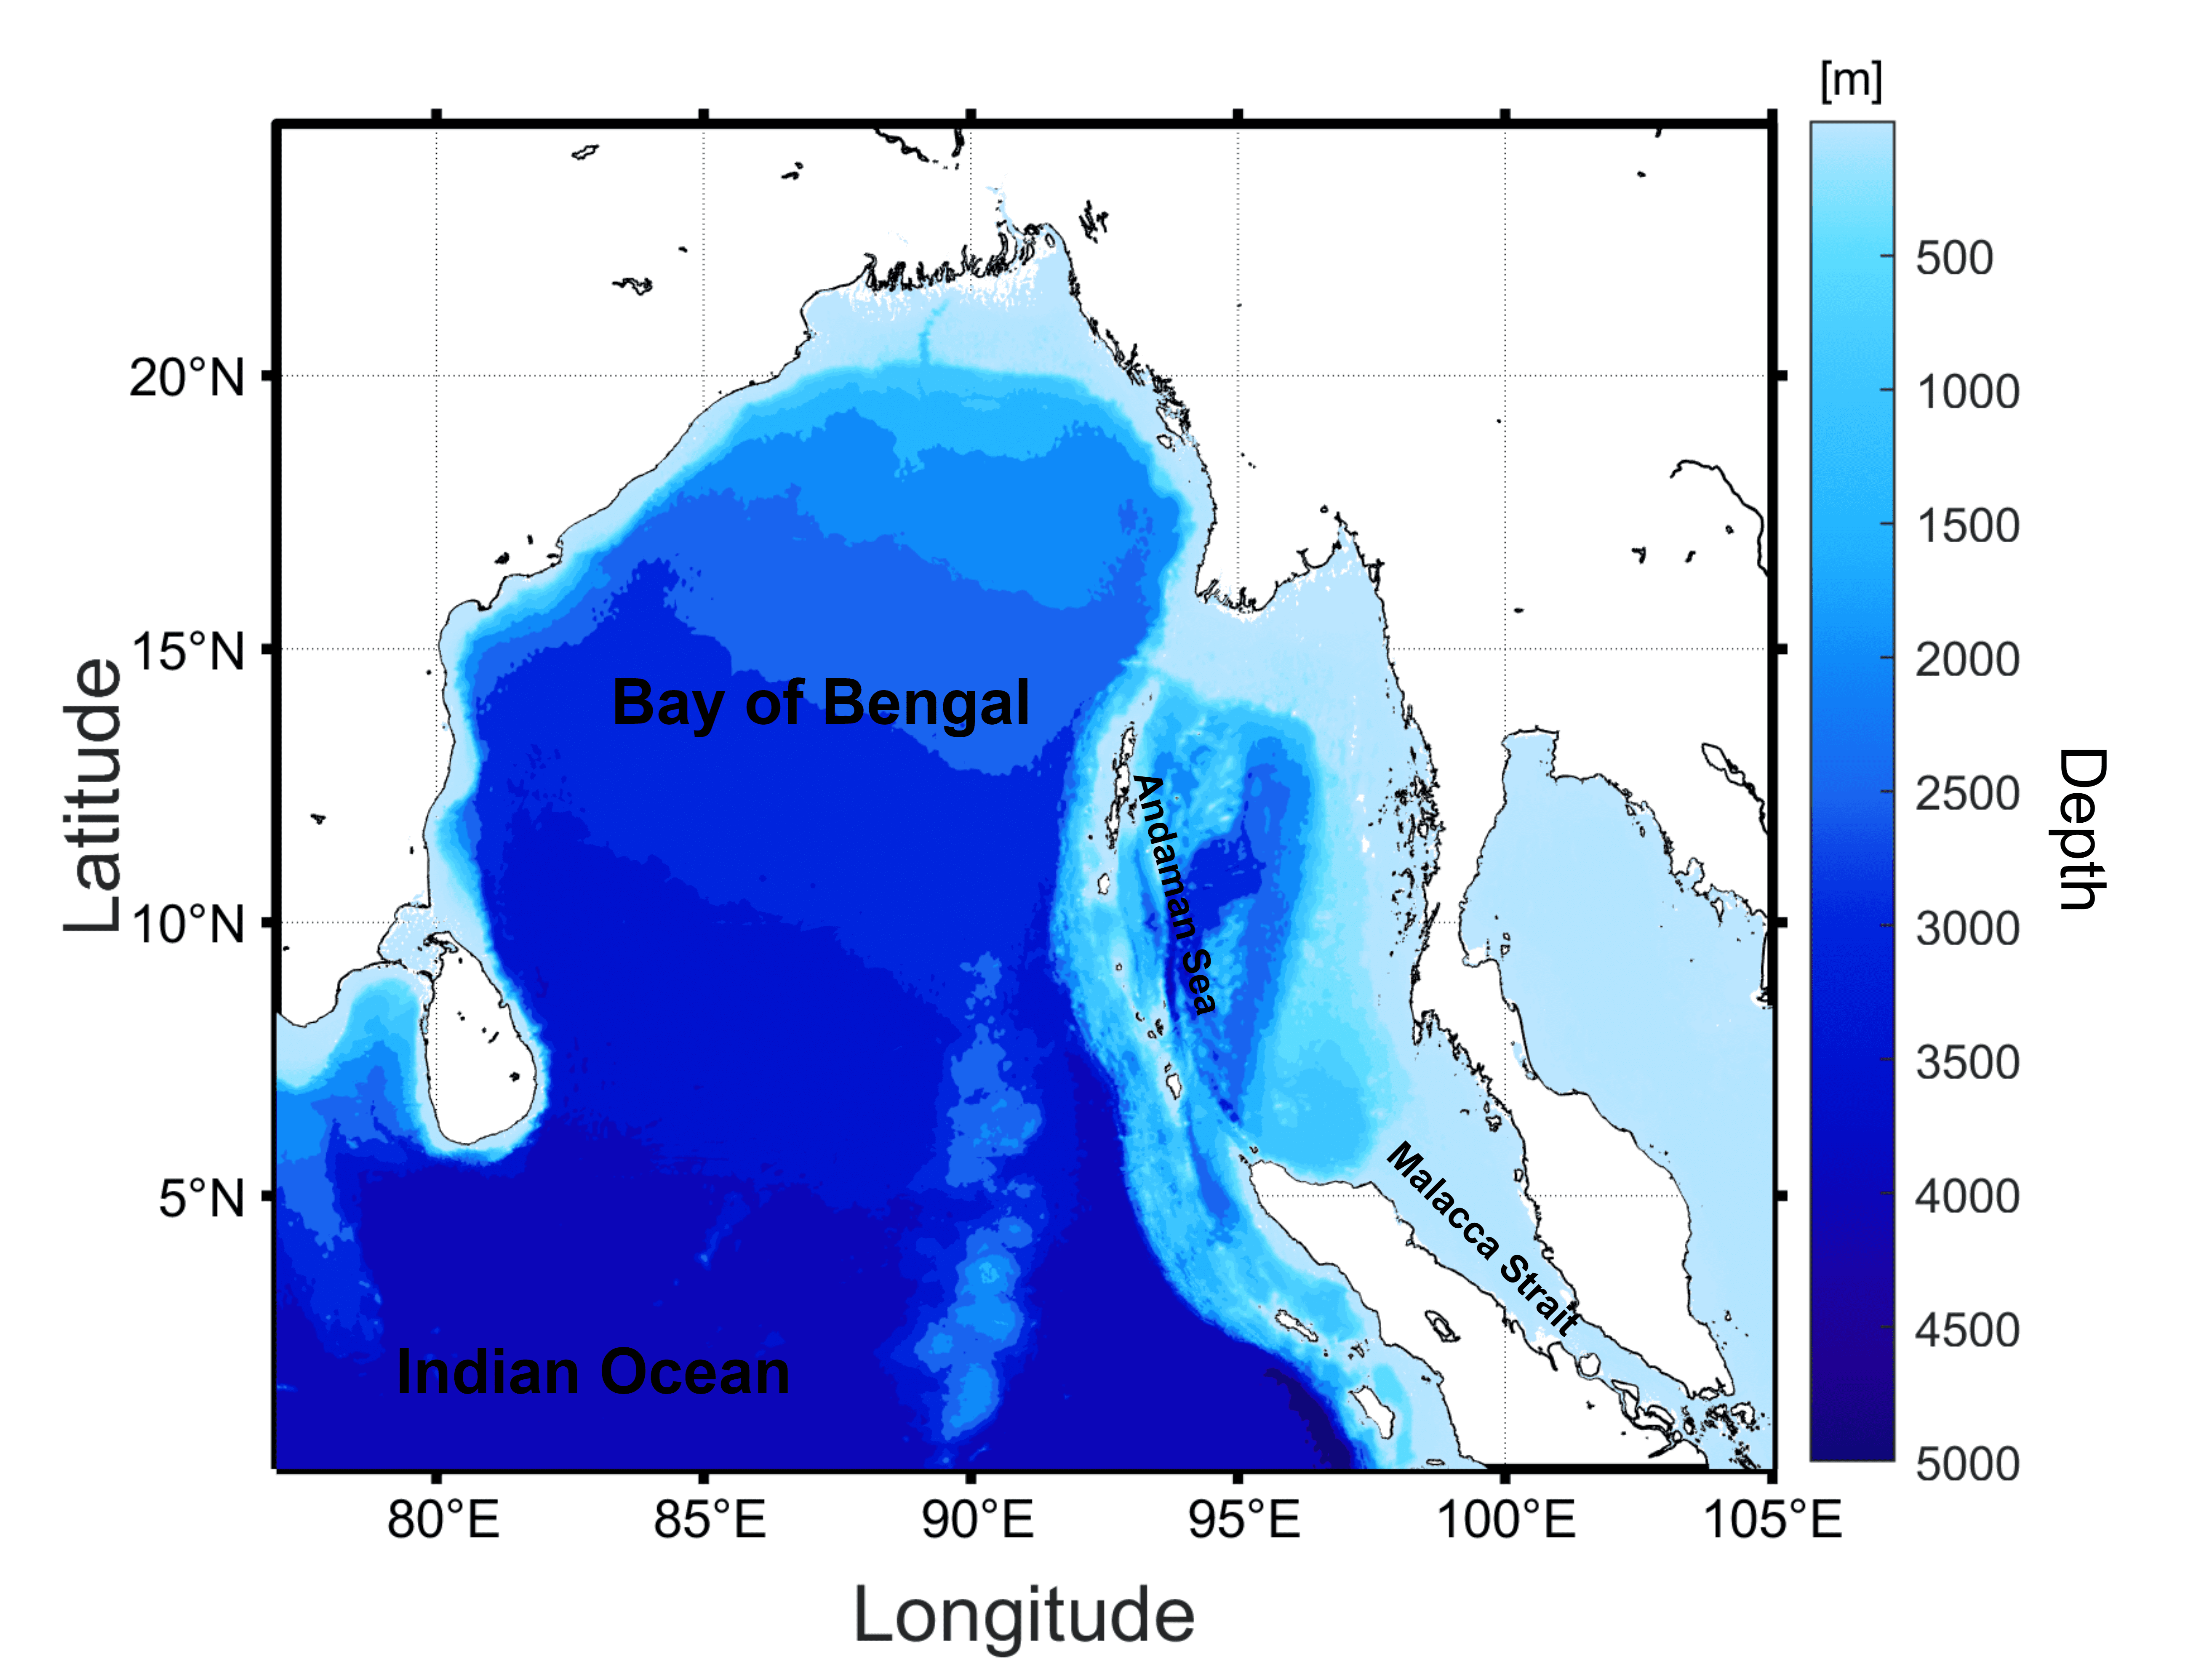
\includegraphics[width=12cm]{contents/Figures/Batimetri_edit_compress}
		\caption{Peta batimetri Samudera Hindia, diperoleh dari SRTM30+ \protect\cite{becker2009global}. Warna dalam peta menunjukkan kedalaman 0-5000 m sedangkan pulau digambarkan tanpa warna.}
		\label{fig:domain}
	\end{figure}
\end{spacing}
\vspace{-0.5pc}
\section[Analisis Data]{Analisis Data}
\begin{spacing}{1.5}
	\subsection[Model Musiman]{Model Musiman}
	 Persamaan siklus musiman \cite{crawley2012r} dapat dituliskan sebagai
	\begin{equation}\label{eq:sm_}
		y = \alpha + \beta \sin(2\pi t)+\gamma \cos(2\pi t) + \epsilon,
	\end{equation}
	dengan $\alpha, \beta$, dan $\gamma$  adalah konstanta pergesaran vertikal, amplitudo dari gelombang sinus, dan amplitudo dari gelombang kosinus. Dalam persamaan ini, $t$ adalah waktu dan $\epsilon$ adalah elemen residual yang mewakili komponen \textit{white-noise} tidak beraturan dalam proses pengambilan data. 
	
	Gambar ini merupakan ilustrasi persamaan \ref{eq:sm_} untuk nilai $\alpha,\beta$ dan $\gamma$ yang berbeda. Nilai $\alpha$ yang berbeda mempengaruhi posisi kurva terhadap sumbu-y. Sedangkan nilai $\beta$ dan $\gamma$ yang berbeda mempengaruhi posisi kurva terhadap sumbu-x.
	\begin{figure}[H]
		\centering
		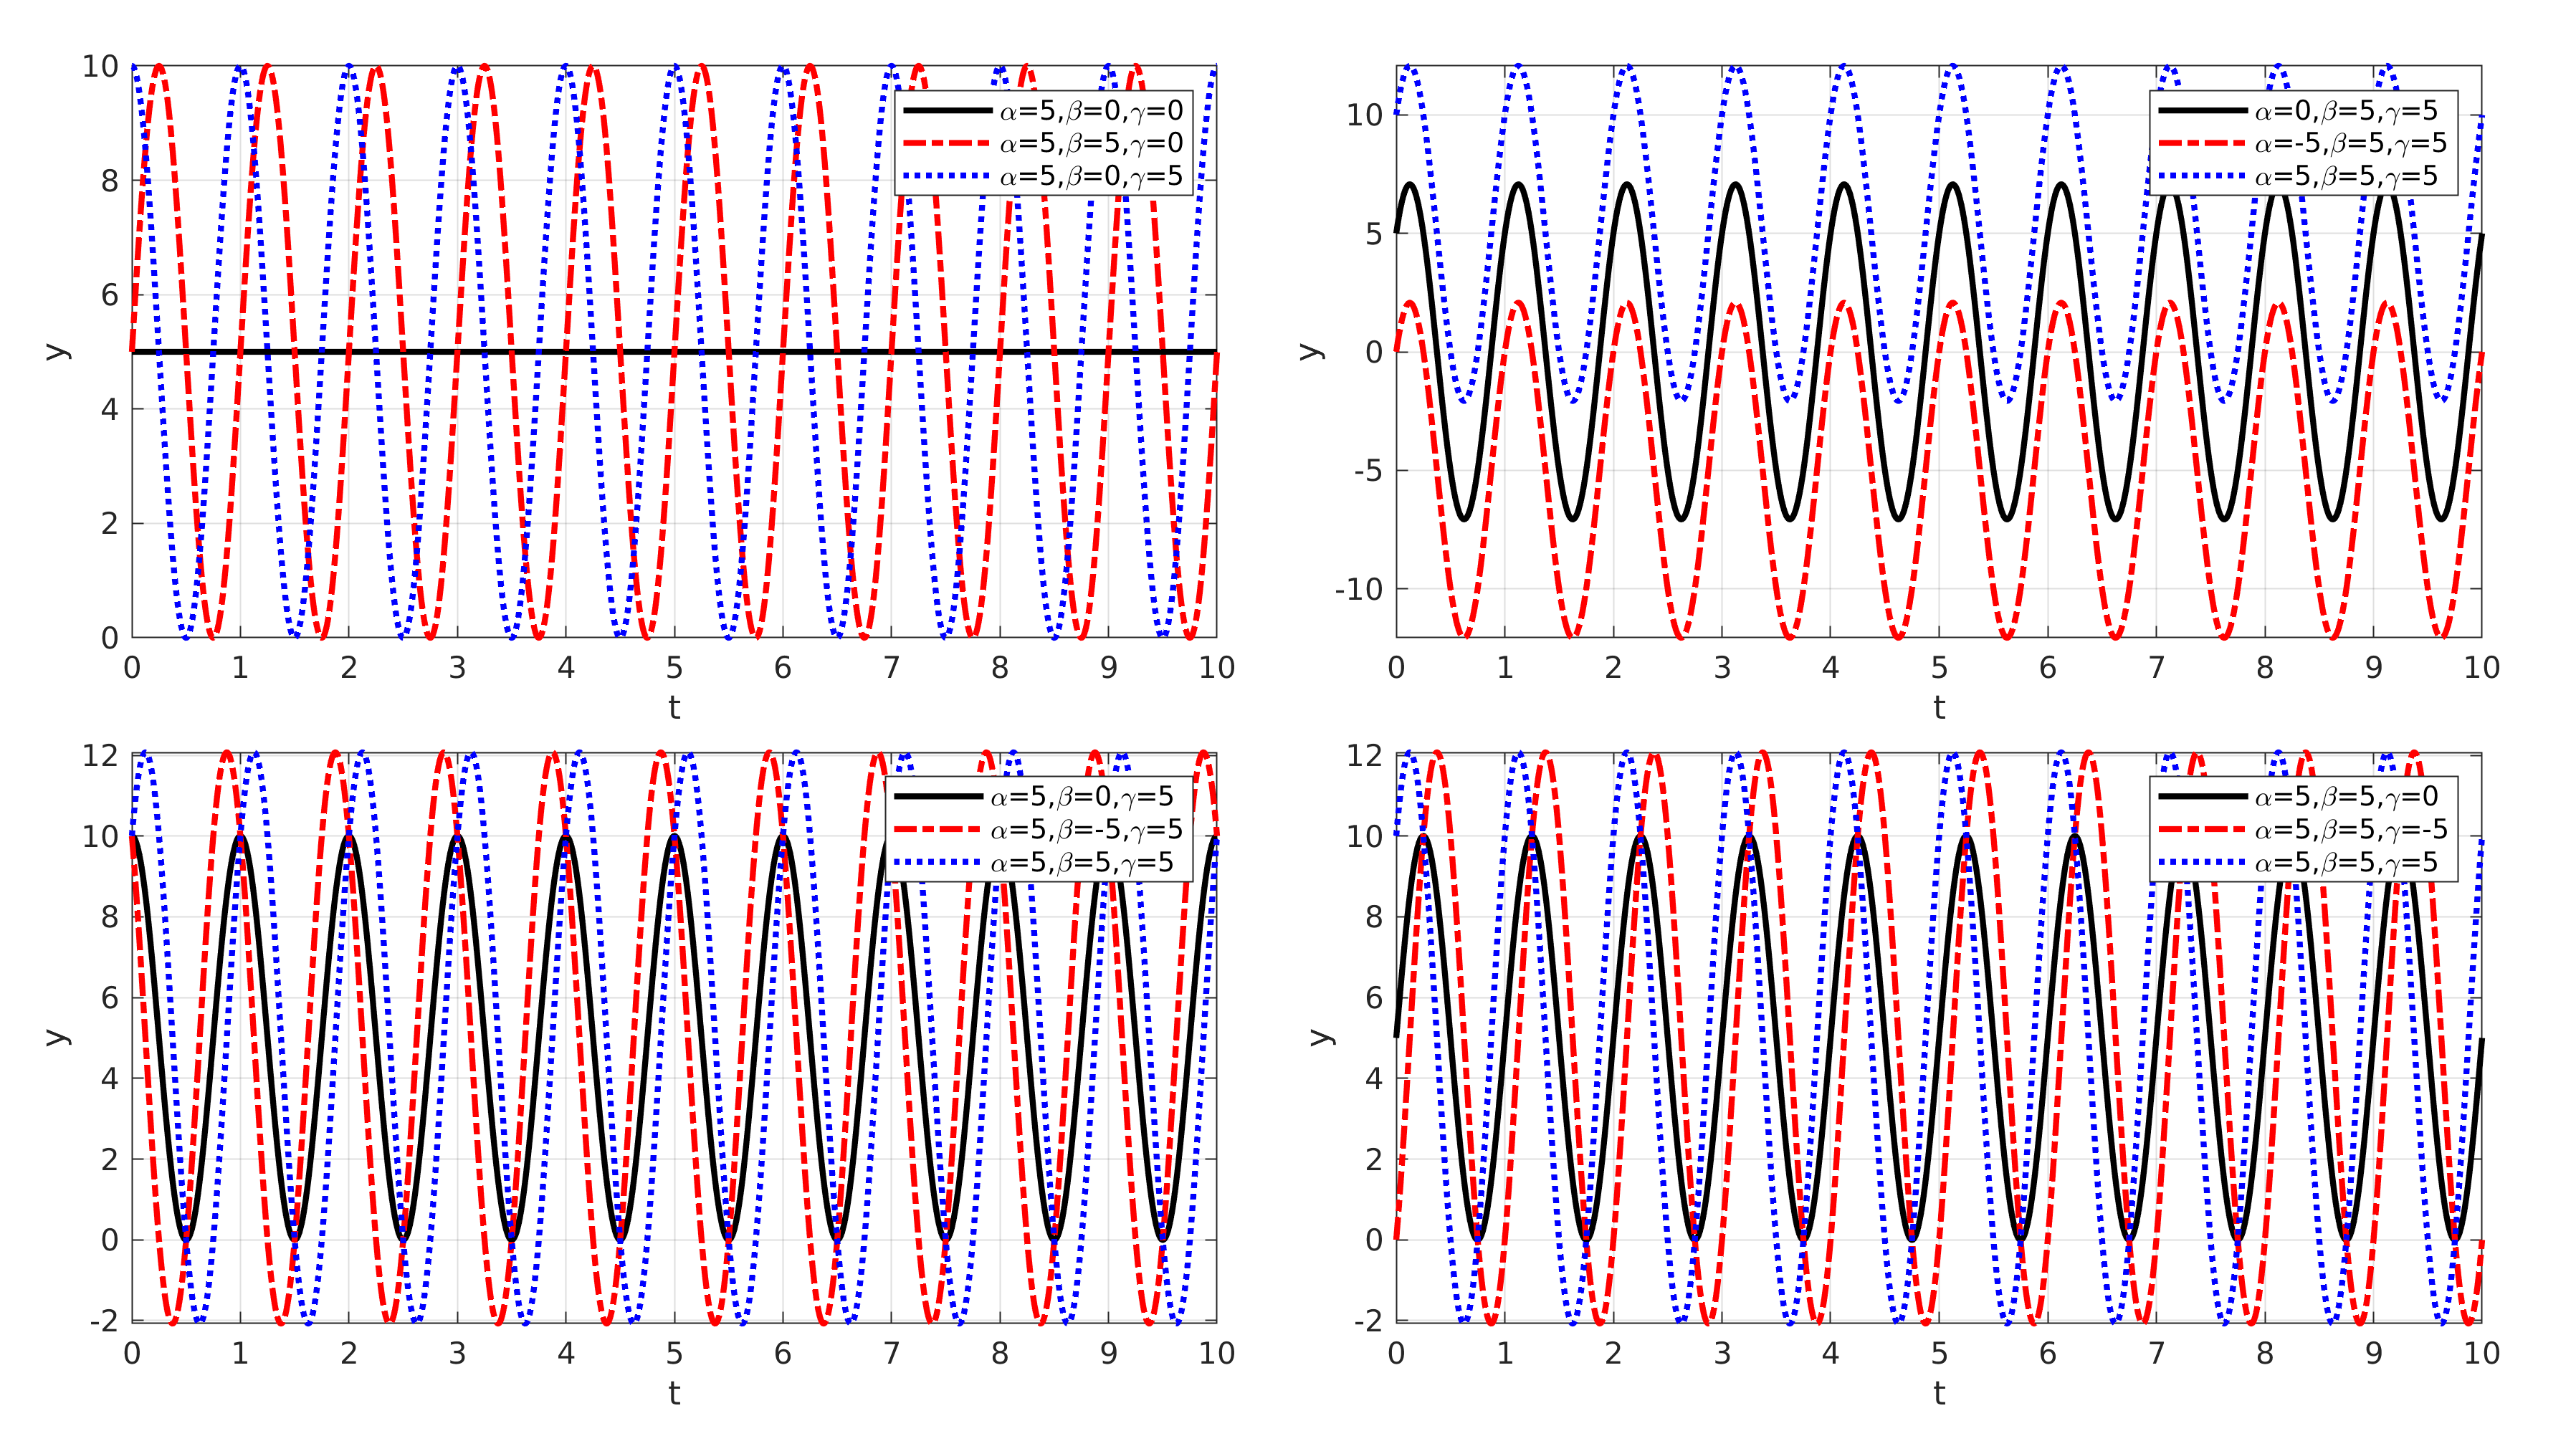
\includegraphics[width=15cm]{contents/Figures/sm_experiment}
		\caption{Ilustrasi persamaan model musiman.}
		\label{fig:sm}
	\end{figure}
	
%	Langkah-langkah yang digunakan untuk menggambarkan \textit{seasonal model} dapat dijelaskan sebagai berikut.
%	\begin{itemize}
%		\item \textbf{\textit{Start}}. \textit{Software} yang digunakan untuk menentukan nilai $\alpha, \beta$ dan $\gamma$ adalah \textit{software} \textit{R}.
%		\item \textbf{\textit{Initialization}}. Dalam proses inisialisasi ini, komponen musiman semua variabel dimodelkan untuk mendapatkan siklus tahunan.
%		\item \textbf{\textit{Input}}. Setelah proses inisialisasi \textit{input} variabel yang ingin diprediksi kemudian dimasukkan.
%		\item \textbf{\textit{Process}}. Selanjutnya dilakukan perhitungan dengan menggunakan fungsi model linear (\verb|lm()|) dalam \textit{R}.
%		\item \textbf{\textit{Output}}. Perintah Summary() digunakan untuk menampilkan hasil dalam proses sebelumnya. Dalam tahapan ini juga diperoleh penggambaran \textit{seasonal model}.
%	\end{itemize}

	\subsection[Analisis Korelasi]{Analisis Korelasi}
		Penelitian ini menganalisis hubungan antara IOD, variabel oseanografi (arus, temperatur, salinitas, MLD, Chl-a, fluks air tawar, fluks panas bersih) dan meteorologi (laju presipitasi dan angin). Persamaan korelasi dan koefisien korelasi yang digunakan dapat dituliskan sebagai \cite{hidayat2023relationship,Haditiar2020}
		\begin{equation}
			\begin{aligned}
				y &= a+rx\\
				r &= \frac{\sum (x_i - \bar{x})(y_i - \bar{y})}{\sqrt{\sum (x_i-\bar{x})^2\sum (y_i-\bar{y})^2}},
			\end{aligned}
		\end{equation}
		dengan $\alpha$ adalah konstanta titik potong sumbu-$y$, $r$ adalah kemiringan dari garis regresi (koefisien regresi), $x_i, y_i$ adalah variable yang digunakan untuk menghitung koefisien korelasi dengan $i$ adalah indeks data. Sedangkan $\bar{x}$ dan $\bar{y}$ adalah rata-rata. 
		
\end{spacing}
\vspace{-0.5pc}
\section[Prosedur Penelitian]{Prosedur Penelitian}
\subsection[Penentuan Kedalaman Lapisan Campuran]{Penentuan Kedalaman Lapisan Campuran}
\begin{spacing}{1.5}
	MLD ditentukan dengan menggunakan data temperatur HYCOM dari hasil penggambaran \textit{cross-section} pada bagian selatan BoB, di latitude 9$^\circ$C, dan bagian utara BoB, di latitude 19$^\circ$C. \textit{Cross-section} temperatur menggunakan kriteria beda hingga, khususnya kriteria nilai \textit{threshold} temperatur, $\Delta t=0.1^\circ$C dengan referensi dari permukaan laut \shortcite{Sprintall1999}. Cara yang digunakan untuk mengestimasi ketebalan MLD adalah dengan cara melihat perubahan temperatur pada setiap kedalaman. Gambar \textit{cross-section} temperatur diplot terlebih dahulu tanpa kontur menggunakan kriteria \textit{threshold} 0.1$^\circ$C untuk menghasilkan gambar dengan warna biru, hijau, dan kuning yang berbeda yang merupakan representasi dari perubahan temperatur. Gambar kontur kemudian ditambahkan untuk melihat secara jelas nilai temperatur berdasarkan interval 1$^\circ$C. Indikator nilai ketebalan MLD berdasarkan perubahan warna dan temperatur yang terjadi pertama kali dari permukaan laut pada gambar.
	
	
	\subsection[Alur Penelitian]{Alur Penelitian}
	Prosedur penelitian mengikuti diagram alir pada Gambar \ref{fig:flowchart} dan dapat dijelaskan sebagai berikut. 
	\begin{itemize}
		\item \textbf{\textit{Start}}. \textit{Software} yang digunakan dalam penelitian ini adalah Matlab dan \textit{R}.
		\item \textbf{\textit{Input}}. Data-data terkait penelitian yang akan digunakan sebagai \textit{input} di\textit{download} terlebih dahulu.
		\item \textbf{\textit{Process}}. Setelah data tersedia, data kemudian diinterpolasi untuk memenuhi data yang kosong serta untuk memperoleh resolusi spasial yang lebih tinggi. Selanjutnya data hasil interpolasi kemudian dibaca dan di konversi ke dalam data matriks pada Matlab. 
		\item \textbf{\textit{Output}}. Hasilnya adalah peta arus, elevasi, temperatur, dan data meteorologi. 
		\item \textbf{\textit{Process}}. Peta temperatur kemudian diobservasi untuk menentukan kedalaman lapisan campuran selama 12 bulan. Selanjutnya, dilakukan analisis model iklim terhadap data meteorologi (\textit{2m air temperature, 2m specific humidity, convective precipitation rate, sea level pressure, wind stress U}, dan \textit{wind stress V}) selama 22 tahun dari tahun 2002 sampai 2021. 
		\item \textbf{\textit{Output}}. Terakhir, diperoleh hasil analisis hubungan MLD dan model iklim.
	\end{itemize}
\end{spacing}
